\chapter{Logische Ausdrücke}\label{ch:K03_logical}

\section{Logische Ausdrücke mit \lstinline|if|, \lstinline|elif| und \lstinline|else|}

\subsection{Logische Ausdrücke mit \lstinline|if|}

\begin{lstlisting}        
note = input("Benoten Sie die Lehrperson (0-100).")
if note == 100:
        print("Echt jetzt? Vielen Dank :)")
\end{lstlisting}

\begin{figure}[H]
\centering
\begin{tikzpicture}[node distance=2cm, transform shape, ->]
    \centering
    
    \node (start) [code] {\lstinline|note = input("Benoten Sie die Lehrperson.")|};
    \node (dec1) [decision, below of=start] {\lstinline|note == 100|};
    \node (print) [code, below of=dec1] {\lstinline|print("Echt jetzt? Vielen Dank :)"|};
    \node (end) [circle,draw=black, fill=black, below of=print, yshift=.5cm] {};
    
    \draw (start) -- (dec1);
    \draw (dec1) -- node[anchor=east] {\lstinline|True|} (print);
    \draw (dec1) --++ (5cm,0cm) |- (end) node[text width=1.5cm, align=left,pos=-0.05] {\lstinline|False|};
    \draw (print) -- (end);
    
\end{tikzpicture}
\end{figure}

\subsection{Logische Ausdrücke mit \lstinline|if| und \lstinline|else|}

\begin{lstlisting}        
note = input("Benoten Sie die Lehrperson (0-100).")
if note == 100:
    print("Echt jetzt? Vielen Dank :)")
else:
    print("Geben Sie mir noch eine Chance")
\end{lstlisting}

\begin{figure}[H]
\centering
\begin{tikzpicture}[node distance=2cm, transform shape, on grid, ->]
    % grid to easier see that the node centers line up while developing plot
    %\draw [help lines] (-5,-9) grid (9,1);
    \node (start) [code] {\lstinline|note = input("Benoten Sie die Lehrperson")|};
    \node (dec1) [decision, below of=start] {\lstinline|note == 100|};
    \node (printif) [code, below left=2cm and 5cm of dec1] {\lstinline|print("Echt jetzt? Vielen Dank :)"|};
    \node (printelse) [code, below right=2cm and 5cm of dec1] {\lstinline|print("Geben Sie mir noch eine Chance"|};
    \node (end) [circle,draw=black, fill=black, below of=dec1, yshift=-2cm] {};
    
    \draw (start) -- (dec1);
    \draw (dec1) -| node[anchor=top, above=.1cm] {\lstinline|True|} (printif);
    \draw (dec1) -| node[anchor=top, above=.1cm] {\lstinline|False|} (printelse);
    \draw (printif) |- (end);
    \draw (printelse) |- (end);
    
\end{tikzpicture}
\end{figure}

\subsection{Logische Ausdrücke mit \lstinline|if|, \lstinline|elif| und \lstinline|else|}
\begin{lstlisting}        
note = input("Benoten Sie die Lehrperson (0-100).")
if note == 100:
    print("Echt jetzt? Vielen Dank :)")
elif note > 60:
    print("Wie kann ich mich noch verbessern?")
else:
    print("Geben Sie mir noch eine Chance")
\end{lstlisting}

\begin{figure}[H]
\centering
\begin{tikzpicture}[node distance=2.5cm, transform shape, on grid, ->]
    % grid to easier see that the node centers line up while developing plot
    %\draw [help lines] (-5,-9) grid (9,1);
    \node (start) [code] {\lstinline|note = input("Benoten Sie die Lehrperson")|};
    \node (dec1) [decision, below of=start] {\lstinline|note == 100|};
    \node (printif) [code, text width=7cm, right=7cm of dec1] {\lstinline|print("Echt jetzt? Vielen Dank :)")|};
    \node (dec2) [decision, below of=dec1] {\lstinline|note > 60|};
    \node (printelif) [code, text width=7cm, right=7cm of dec2] {\lstinline|print("Wie kann ich mich noch verbessern?")|};
    \node (printelse) [code, text width=6cm, below of=dec2] {\lstinline|print("Geben Sie mir noch eine Chance")|};
    \node (end) [circle,draw=black, fill=black, below of=printelse, yshift=.8cm] {};
    
    \draw (start) -- (dec1);
    \draw (dec1) -- node[anchor=top, above=.1cm] {\lstinline|True|} (printif);
    \draw (dec1) -- node[anchor=east] {\lstinline|False|} (dec2);
    
    \draw (dec2) -- node[anchor=top, above=.1cm] {\lstinline|True|} (printelif);
    \draw (dec2) -- node[anchor=east] {\lstinline|False|} (printelse);
    
    \draw (printif) --++ (4.5cm,0cm) |- (end);
    \draw (printelif) --++ (4.5cm,0cm) |- (end);
    
    \draw (printelse) -- (end);
    
\end{tikzpicture}
\end{figure}

\begin{myexercise}
Wo liegt hier das Problem?
\begin{lstlisting}        
note = input("Benoten Sie die Lehrperson (0-100).") 
# wir tippen 100 in das Fenster ein

if note == 100:
    print("Echt jetzt? Vielen Dank :)")
if note > 60:
    print("Wie kann ich mich noch verbessern?")
else:
    print("Geben Sie mir noch eine Chance")
\end{lstlisting}
\end{myexercise}

\section{Fussgesteuerte Schleifen mit \lstinline|break|}
Bisher haben wir eine Art von Schleife gesehen: \lstinline|for _ in range(...)|. Dabei gibt die Zahl innerhalb des Befehls \lstinline|range(...)| an, wie viele Mal der Schleifenkörper wiederholt wird. Manchmal wissen wir jedoch nicht im voraus, wie viele Male eine Schleife wiederholt werden soll, wir kennen jedoch eine Bedingung, bei der die Schleife abgebrochen werden soll. Dies könnte beispielsweise der Fall sein, wenn wir eine Spirale zeichnen wolle, die immer grösser wird, bis die Seitenlänge eine gewisse maximale Länge \lstinline|max_seite| erreicht hat.



\begin{figure}[H]
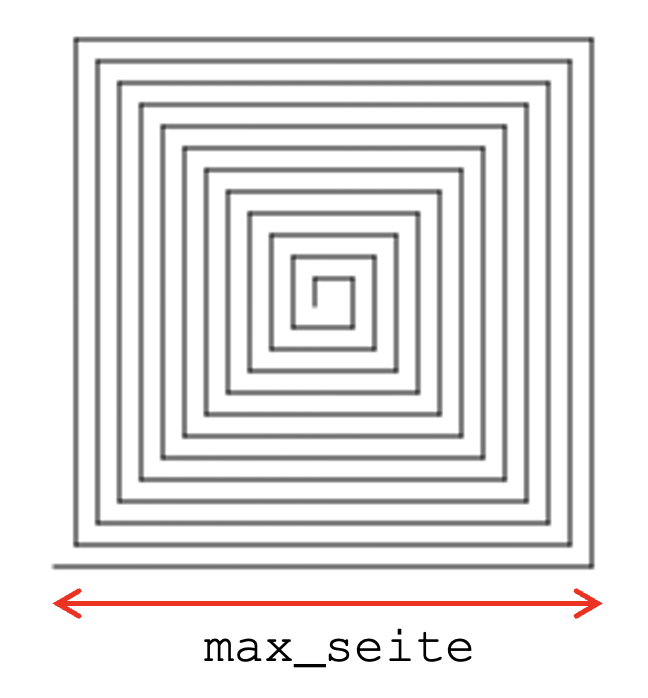
\includegraphics[width=.2\linewidth]{GrundlagenInfo/00_Programmieren/Figures/spirale_while}
\end{figure}

Natürlich könnte man auch hier berechnen, wie viele Male die \lstinline|for|-Schleife ausgeführt werden muss. Die Formel, um dies zu berechnen, wäre:
\[\floor{\frac{\text{\texttt{maxseite - seite}}}{\text{\texttt{add}}}} + 1\]

Es geht allerdings auch einfacher, indem wir eine ``unendliche'' Schleife starten, die wir abbrechen, sobald eine gewisse Kondition wahr ist.


\begin{lstlisting}[escapechar=!]
import turtle as t

# Tempo der Turtle festlegen
t.speed(100)

# gleichseitiges Dreieck zeichnen
seite = 5
max_seite = 50
increment = 5
while True:!\tikzmark{repeatFrom}!                            !\tikzmark{repeat}!
    if seite > max_seite:
        break!\tikzmark{breakFrom}!                       !\tikzmark{break}!
    t.fd(seite)
    t.rt(90)
    seite += increment

# Turtle-Zeichnung stehen lassen
t.done()
\end{lstlisting}

%\lstinputlisting[language=Python,caption=\texttt{spirale.py},label=listing:spirale]{GrundlagenInfo/00_Programmieren/Skript/Code/K03_Logic/spirale.py}

\begin{tikzpicture}[overlay, remember picture,
    every node/.style={draw=red!50,fill=red!50!white,text=black,rounded corners}]
    \drawArrow{repeatFrom}{repeat}{\footnotesize Unendliche Schleife}{DeepPink};
    \drawArrow{breakFrom}{break}{\footnotesize Schleifenabbruch}{DeepPink};
\end{tikzpicture}

\section{Kopfgesteuerte Schleifen mit \lstinline|while|}

\begin{minipage}{.45\textwidth}
\begin{lstlisting}[escapechar=!]
import turtle as t

def spirale(seite, add, max_seite):
    while True:               !\tikzmark{fromStart}!
    	if seite > max_seite:
    	    break             !\tikzmark{fromEnd}!
        t.fd(seite)
        t.rt(90)
        seite+=add

spirale(10, 10, 100)
\end{lstlisting}
\end{minipage}
\begin{minipage}{.45\textwidth}
\begin{lstlisting}[escapechar=!]
import turtle as t

def spirale(seite, add, max_seite):
    !\tikzmark{toStart}!!\tikzmark{toEnd}!while seite > max_seite:
        t.fd(seite)
        t.rt(90)
        seite+=add
        
spirale(10, 10, 100)
\end{lstlisting}
\end{minipage}
\begin{tikzpicture}[overlay, remember picture,
    every edge/.append style = { ->, thick, >=stealth, red!70},
    every node/.style={draw=red!50,fill=red!50!white,text=black,rounded corners}]
	
	\drawBrace{0em}{fromStart}{fromEnd}{}{.5}{}{}
	\drawBrace{-.5em}{toStart}{toEnd}{}{.5}{mirror}{}
	% arrow pointing from one code to other
	\draw[->, style={thick, >=stealth, red!70}] (fromStartfromEnd-coord-arrow) to (toStarttoEnd-coord-arrow);
\end{tikzpicture}


\begin{myattention}[Endlos-Schleifen]
Beachten Sie folgende Punkte:
\begin{itemize}
\item Passen Sie auf, dass Sie keine unendlichen Schleifen produzieren! In diesem Fall kann das Programm, auf dem Python läuft, hängen bleiben. Vergessen Sie daher nie die Abbruchkondition klar zu formulieren!
\item Ein \lstinline|while True:| (unendliche Schleife) ohne \lstinline|break| kann zum Absturz des Programms führen \emoji{face-with-spiral-eyes}
\item Je nachdem kann das auch in einem \lstinline|while| mit einer Kondition passieren, sofern die Bedingung nach dem \lstinline|while| so geschrieben ist, dass sie immer wahr (\lstinline|True|) ist (s. \cref{subsec:semantische-fehler} zu semantischen Fehlern).
\item \textbf{Speichern Sie regelmässig Ihre Aufgaben!}
\item Falls das Programm VSCodium hängenbleibt: Beenden mit \keys{Ctrl+Alt+\backdel} (Windows), bzw. Activity Monitor unter MacOS
\end{itemize}
\end{myattention}

\section{Bool'sche Ausdrücke}
\begin{itemize}
    \item \tib{Boolsche Ausdrücke} sind Ausdrücke, die genau zwei verschiedene Werte annehmen können: entweder \textit{wahr} (\lstinline|True|) oder \textit{falsch} (\lstinline|False|). Beispiele:
    \begin{itemize}
        \item \lstinline|3 == 5 # False|
        \item \lstinline|(9 + 3) < (2 * 8) # True|
    \end{itemize}
    \item Weitere boolsche Relationen:
    \begin{table}[H]
        \centering
        \footnotesize
        \begin{tabular}{c||p{3.1cm}}
        \textbf{Python} & \textbf{Mathematische\newline Bedeutung} \\\midrule 
             \lstinline|==| & gleich ($=$)\\
             \lstinline|!=| & ungleich ($\neq$) \\
             \lstinline|<| & kleiner ($<$)\\
             \lstinline|<=| & kleiner oder gleich ($\leq$) \\
             \lstinline|>| & grösser ($>$) \\
             \lstinline|>=| & grösser oder gleich ($\geq$)
        \end{tabular}
    \end{table}
    \item Verwendungsart
\begin{lstlisting}
if BOOLSCHER_AUSDRUCK:
    # dieser Code wir höchstens dann ausgeführt, wenn 
    # BOOLSCHER_AUSDRUCK wahr ist (True)
\end{lstlisting}
\end{itemize}

\begin{itemize}
    \item \tib{Boolsche Ausdrücke} sind Ausdrücke, die genau zwei verschiedene Werte annehmen können: entweder \textit{wahr} (\lstinline|True|) oder \textit{falsch} (\lstinline|False|). Beispiele:
    \begin{itemize}
        \item \lstinline|3 == 5 # False|
        \item \lstinline|(9 + 3) < (2 * 8) # True|
    \end{itemize}
    \item Weitere boolsche Relationen:
    \begin{table}[H]
        \centering
        \footnotesize
        \begin{tabular}{c|c||p{3.1cm}}
        \textbf{(SQL)} &\textbf{Python} & \textbf{Mathematische\newline Bedeutung} \\\midrule 
             \lstinline[style=sql]|=|&\lstinline|==| & gleich ($=$)\\
             \lstinline[style=sql]|<>|&\lstinline|!=| & ungleich ($\neq$) \\
             \lstinline[style=sql]|<|&\lstinline|<| & kleiner ($<$)\\
             \lstinline[style=sql]|<=|&\lstinline|<=| & kleiner oder gleich ($\leq$) \\
             \lstinline[style=sql]|>|&\lstinline|>| & grösser ($>$) \\
             \lstinline[style=sql]|>=|&\lstinline|>=| & grösser oder gleich ($\geq$)
        \end{tabular}
    \end{table}
    \item Verwendungsart
\begin{lstlisting}
if BOOLSCHER_AUSDRUCK:
    # dieser Code wir höchstens dann ausgeführt, wenn 
    # BOOLSCHER_AUSDRUCK wahr ist (True)
\end{lstlisting}
\end{itemize}

Lösen Sie folgende Aufgaben:
\begin{itemize}
    \item Lesen Sie Beispiel 4.1
    \item \aufgabebox{Aufgaben 4.3, 4.6}
    \item \abgabebox{Aufgabe 4.8 $\rightarrow$ Abgabe}
    \item \abgabebox{Aufgabe 4.11 $\rightarrow$ Abgabe}
    \item \aufgabebox{Aufgaben 4.12 - 4.14}
    \item \challengebox{``Dynamisches Schachbrett'' (Moodle)}
\end{itemize}